\documentclass[a4paper, 10pt]{article}
\usepackage[utf8]{inputenc}
\usepackage{amsmath}
\usepackage{amssymb}
\usepackage{amsthm}
\usepackage{amsfonts}
\usepackage{BOONDOX-cal}
\usepackage{quiver}
\usepackage[a4paper, margin=1in]{geometry}
\usepackage{tikz}
\usepackage{tikzscale}
\usepackage{subcaption}
\usepackage{wrapfig}
\usepackage{multicol}
\usepackage{parskip}
\usepackage{hyperref}
\usepackage{biblatex}

\newcommand{\ran}{\textrm{Range}\,}
\newcommand{\bbN}{\mathbb{N}}
\newcommand{\bbR}{\mathbb{R}}
\newcommand{\bbC}{\mathbb{C}}

\newcommand{\ob}{\text{ob}}
%\newcommand{\hom}{\text{Hom}}
\newcommand{\id}{\text{id}}

%\newcommand{\sA}{\boldsymbol{\mathcal{A}}}
%\newcommand{\sB}{\boldsymbol{\mathcal{B}}}
\newcommand{\sA}{\mathbcal{A}}
\newcommand{\sB}{\mathbcal{B}}

\newcommand{\T}{\mathcal{T}}
\newcommand{\bT}{\mathbcal{T}}
\newcommand{\mettop}{\mathbcal{MetTop}}

\theoremstyle{definition}
\newtheorem{definition}{Definition}[section]
\def\definitionautorefname{Definition}

\newtheorem{theorem}[definition]{Theorem}
\def\theoremautorefname{Theorem}
\newtheorem{proposition}[definition]{Proposition}
\def\propositionautorefname{Proposition}
\newtheorem{lemma}[definition]{Lemma}
\def\lemmaautorefname{Lemma}
\newtheorem{corollary}[definition]{Corollary}
\def\corollaryautorefname{Corollary}

\theoremstyle{remark}
\newtheorem*{remark}{Remark}
\def\remarkautorefname{Remark}

\theoremstyle{remark}
\newtheorem{example}[definition]{Example}
\def\exampleautorefname{Ex.}

\addbibresource{handout.bib}

\title{\vspace*{-5ex}
       A Categorical Introduction to Dynamical Systems \\
       {\large Functors, Natural Transformations, Category of Functors, Equivalence of Categories }
}

\author{\vspace*{-15ex}April Herwig}
\date{02.11.2023}

\begin{document}

\maketitle

% --------------------------------------------------

\section{Two Dynamical Systems}

\begin{figure}[h!]
    \begin{subfigure}{0.5\textwidth}
        \centering
        \begin{tikzpicture}[scale=0.6]
            \node (0) at (0, 0) {};
            \node (1) at (4.25, 0) {};
            \node (2) at (0, 4.25) {};
            \node (4) at (4, 0) {};
            \node (5) at (2, 4) {};
            \node (6) at (-0.25, 4) {};
            \node (7) at (0.25, 4) {};
            \node (8) at (4, 0.25) {};
            \node (9) at (4, -0.25) {};
            \node (10) at (-0.75, 4) {$1$};
            \node (11) at (4, -0.75) {$1$};
            \node (12) at (-0.25, -0.25) {$0$};
            \node (13) at (3, 3.5) {{\color{purple} $\phi_1$}};
            \draw (2.center) to (0.center);
            \draw (0.center) to (1.center);
            \draw[purple] (0.center) to (5.center);
            \draw[purple] (5.center) to (4.center);
            \draw (6.center) to (7.center);
            \draw (9.center) to (8.center);
        \end{tikzpicture}
        \caption{Tent map}
    \end{subfigure}%
    \begin{subfigure}{0.5\textwidth}
        \centering
        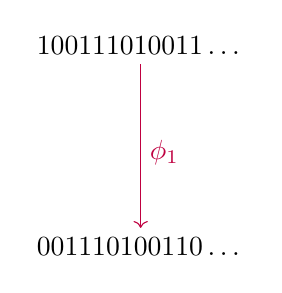
\begin{tikzpicture}[scale=0.6]
            \node (0) at (0, 4.25) {$100111010011\dots$};
            \node (1) at (0, 0) {$001110100110\dots$};
            \node (2) at (0.5, 2) {{\color{purple} $\phi_1$}};
            \draw[->, purple] (0) to (1);
        \end{tikzpicture}
        \caption{Left shift map on two symbols}
    \end{subfigure}
\end{figure}

%\clearpage

\section{Functors}

\begin{definition}
    A \emph{functor} $F : \sA \to \sB$ between two categories $\sA$ and $\sB$ maps $\ob (\sA) \to \ob (\sB)$, $\hom_{\sA} \to \hom_{\sB}$ in the following structure-preserving way:

    \begin{itemize}
        \item for all $A \in \ob (\sA)$, $F(\id_A) = \id_{F(\sA)}$;
        \item for all $A_1, A_2, A_3 \in \ob (\sA)$, the diagram commutes
            % https://q.uiver.app/#q=WzAsMyxbMiwwLCJGKEFfMikiXSxbMiwyLCJGKEFfMykiXSxbMCwwLCJGKEFfMSkiXSxbMCwxLCJGKGYpIl0sWzIsMSwiRihnIFxcY2lyYyBmKSIsMl0sWzIsMCwiRihnKSJdXQ==
            \[\begin{tikzcd}
                {F(A_1)} && {F(A_2)} \\
                \\
                && {F(A_3)}
                \arrow["{F(f)}", from=1-3, to=3-3]
                \arrow["{F(g \circ f)}"', from=1-1, to=3-3]
                \arrow["{F(g)}", from=1-1, to=1-3]
            \end{tikzcd}\]
    \end{itemize}
\end{definition}

\begin{example}
    A \emph{dynamical system} is a functor $\phi$ from an additive semigroup $\bT$ (viewed as a single-object category) to the category $\mettop$ of metrizable spaces with continuous functions. 
\end{example}

\section{Natural Transformations}

\begin{definition}
    A \emph{natural transformation} is a morphism in the category $[\sA , \sB]$ of functors from $\sA$ to $\sB$. Specifically, a natural transformation (\emph{natural morphism, natural isomorphism, etc.}) is a collection $\left\{ \eta_A \right\}_{A \in \ob (\sA)}$ of morphisms such that 

    \begin{itemize}
        \item for all $A_1, A_2 \in \ob (\sA)$ and $f: A_1 \to A_2$, the diagram commutes
            % https://q.uiver.app/#q=WzAsNCxbMCwwLCJGKEFfMSkiXSxbMiwwLCJGKEFfMikiXSxbMiwyLCJHKEFfMiJdLFswLDIsIkcoQV8xKSJdLFswLDEsIkYoZikiXSxbMSwyLCJcXGV0YV97QV8yfSJdLFswLDMsIlxcZXRhX3tBXzF9IiwyXSxbMywyLCJHKGYpIiwyXV0=
            \[\begin{tikzcd}
                {F(A_1)} && {F(A_2)} \\
                \\
                {G(A_1)} && {G(A_2)}
                \arrow["{F(f)}", from=1-1, to=1-3]
                \arrow["{\eta_{A_2}}", from=1-3, to=3-3]
                \arrow["{\eta_{A_1}}"', from=1-1, to=3-1]
                \arrow["{G(f)}"', from=3-1, to=3-3]
            \end{tikzcd}\]  
    \end{itemize}

    We write $\eta: F \implies G$, and write $\sA \cong \sB$ if there exists a natural isomorphism $\eta$. 
    
    Moreover, if two functors $F: \sA \to \sB$, $G: \sB \to \sA$ satisfy $G \circ F \cong \id_{\sA}$, $F \circ G \cong \id_{\sB}$, then we say $\sA$ and $\sB$ are \emph{equivalent}, write $\sA \simeq \sB$. 
\end{definition}

\begin{example}
    Given two dynamical systems, that is two functors $\phi, \psi :  \bT \to \mettop$, a homeomorphism $h$ which satisfies $\psi_1 = h^{-1} \circ \phi_1 \circ h$ is known in dynamical systems literature as a \emph{topological conjugacy}. Such a homeomorphism is precisely a natural isomorphism when viewed in the categorical context. 
\end{example}

\begin{example}
    The tent map is topologically conjugate to the left shift on two symbols. The conjugacy is constructed using a so-called "itinerary map" technique. Systems which are conjugate share many properties, including \emph{chaos}. This is to say, despite how simple the map looks - a piecewise linear map - after just a few iterations the dynamics become incalculably complicated!
\end{example}

\section{Equivalence}

\begin{theorem}
    A functor $F: \sA \to \sB$ induces an equivalence of categories $\sA \simeq \sB$ if and only if $F$ is
    \begin{itemize}
        \item \emph{fully faithful}: for all $A_1, A_2 \in \ob (\sA)$, the map $f \mapsto F(f)$ is a bijection 
        \begin{equation*}
            \hom_{\sA} (A_1, A_2) \to \hom_{F(\sA)} (F(A_1), F(A_2)) ;
        \end{equation*}
        \item \emph{essentially surjective}: every $b \in \ob (\sB)$ is isomorphic to some $F(A)$, $A \in \ob (\sA)$. 
    \end{itemize}
\end{theorem}

% --------------------------------------------------

\nocite{*}
\printbibliography

\end{document}
